\documentclass[a4paper]{article}

\usepackage[french]{babel}
\usepackage[utf8x]{inputenc}
\usepackage{amsmath}
\usepackage{graphicx}
\usepackage[colorinlistoftodos]{todonotes}
\usepackage{amsfonts}
\usepackage[T1]{fontenc}
\usepackage{listings}

\title{TP1 \\ Acquisition de connaissances 2}

\author{Damien Crémilleux - Lauriane Holy}

\date{\today}



\begin{document}
\maketitle


\section{Apprentissage d'un SVM}

\begin{enumerate}


\item On constate sur la figure~\ref{fig:capture1} que les points négatifs et positifs sont séparables linéairement par plusieurs droites.
	

\begin{figure}[h]
 	 \begin{center}	
 	   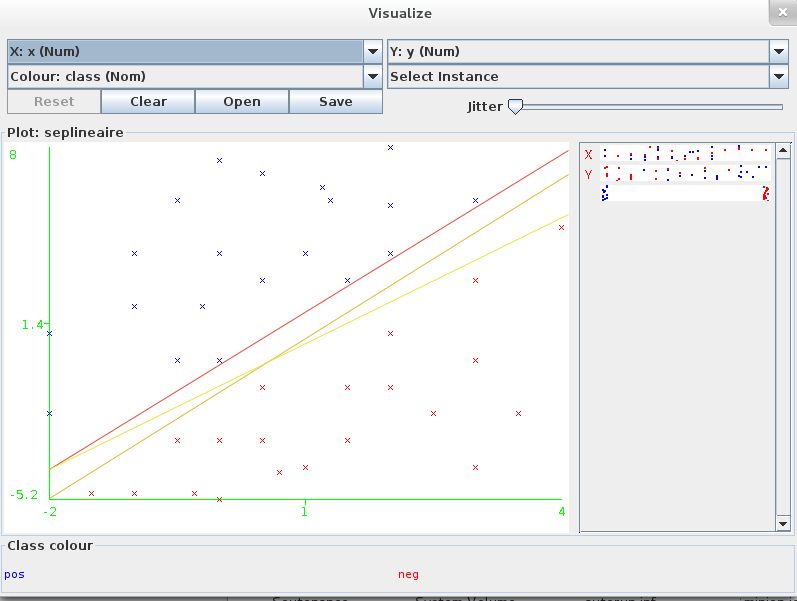
\includegraphics[width=0.8\textwidth]{Capture1.png}
 	   \caption{Visualisation des données SepLineaire.arff et droites séparatrices}
 	   \label{fig:capture1} 
 	 \end{center}
	\end{figure}

\item Après avoir séparé le jeu de données en un jeu d'apprentissage et de test et effectué une SMO, nous obtenons l'équation cartésienne de droite suivante : 1.4531x - 0.8174y + 0.7266.

La valeur du risque empirique est de 0. Ceci s'explique par le fait que les données d'entrainement et de test sont les mêmes, il s'agit d'un apprentissage par coeur.

\item L'utilisation de \textit{TrainTestSplitMaker} permet d'avoir 66\% des données utilisées pour l'apprentissage et le reste pour le test. On obtient alors l'équation suivante : 1.4533x - 0.8175 + 0.7266 et un risque empirique de 0 également.

L'utilisation de \textit{CrossValidationFoldMaker} permet, quant-à lui, de prendre une partie des données, divisées en 10 ici, pour le test et le reste pour l'entrainement, puis de prendre une nouvelle partie pour le test et continuer ainsi 10 fois.
Le résultat de cette utilisation permet d'obtenir une moyenne des classifieurs et d'obtenir une bonne estimation. Ici également, toutes les instances ont bien été classées.

Ici, de façon exceptionnelle nous obtenons un risque empirique de 0, le classifieur ne fait aucune erreur sur le jeu de test.

\end{enumerate}


\subsection{Données non linéairement séparables}

On cherche les paramètres permettant de mieux apprendre les données d'apprentissage.

\begin{tabular}{ |c|c|c| }
  \hline
  Algorithme & Nombre de vecteurs de supports & Nombre d'erreurs \\ \hline
  NormalizePolyKernel & 62  & 6 \\
  PolyKernel & no &  14 \\
  Puk & 32 & 0\\
  RBFKernel & 64 & 15\\
  StringKernel & 64 & 15 \\  
  \hline
\end{tabular}

Le meilleur résultat est donc obtenu pour l'algorithme Puk. Celui-ci requiert 32 vecteurs de supports.


\section{Apprentissage d'un arbre de décision}
\subsection{Construction et évaluation d'arbres}
\begin{enumerate}

\item
 Il y a 14 instances caractérisées par 5 attributs : 
	\begin{itemize}
		\item \textit{outlook} : nominal 	
		\item \textit{temperature} : nominal 
		\item \textit{humidity} : binaire
		\item \textit{windy} : binaire
		\item \textit{play} : binaire, la classe.
	\end{itemize}
	La classe à prédire est si l'on peut jouer ou non en fonction de ces différents attributs (\textit{concept learning}).


\item
	L'arbre de décision obtenu avec un jeu de donnée utilisant 66\% des données pour l'apprentissage et le reste pour le test est représenté en figure~\ref{fig:Arbre}.

	\begin{figure}[h]
	  \begin{center}
	    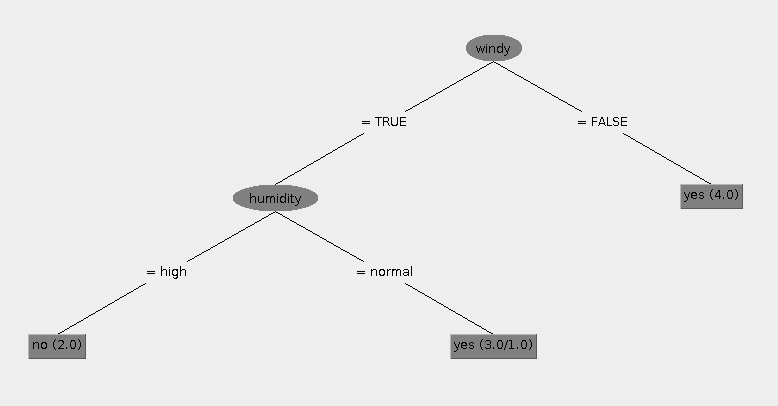
\includegraphics[width=0.8\textwidth]{ArbreInit.png}
	    \caption{Arbre de décision}
	    \label{fig:Arbre} 
	  \end{center}
	\end{figure}

On constate que 3 instances sur 5 ont été mal classées et que l'apprentissage est moins efficace pour la valeur \textit{play = no}.

\item 
En faisant varier la graine utilisée on constate que le nombre d'instances mal classées varie. En effet, la graine permet de prendre les exemples de façon aléatoire, la changer revient à prendre un autre ensemble d'exemples pour l'entrainement. 

Plus le pourcentage d'utilisation des exemples en tant que données d'apprentissage est élevé plus l'erreur est importante. En effet, cela signifie que le classifieur va trop apprendre des exemples. De même, si le pourcentage est trop faible, le taux d'erreur sera également plus important car le classifieur sera trop général et n'apprendra pas assez. Il faut trouver un juste équilibre.

Dans notre cas, étant donné le faible nombre d'exemples, la génération du classifieur via la partition des données en entrainenement et test n'est pas concluante.

\item Dans le fichier \textit{weather.arff}, les attributs \textit{temperature} et \textit{humidity} ont été remplacés par des attributs numériques de $\mathbb{R}$ (à la place de nominaux).

Au niveau des résultats de test il n'y a pas de changement. 


Au niveau de l'algorithme il est nécessaire de mettre un seuil, comme le montre l'arbre en figure~\ref{fig:ArbreSeuil} où un seuil à 80 pour l'attribut \textit{humidity} a été mis en place.
Les exemples sont triés suivant la valeur des attributs \textit{humidity} et \textit{temperature} puis le seuil choisit est celui qui minimise l'entropie.


Il y a donc ici plusieurs attributs numériques de $\mathbb{R}$, l'idée, dans l'algorithme, est donc de les regrouper et d'obtenir une découpe oblique composé des séparatrices linéaires des ces attributs. Ainsi, on compare une combinaison de ces attributs par rapport à ce nouveau seuil.

\begin{figure}[h]
	  \begin{center}
	    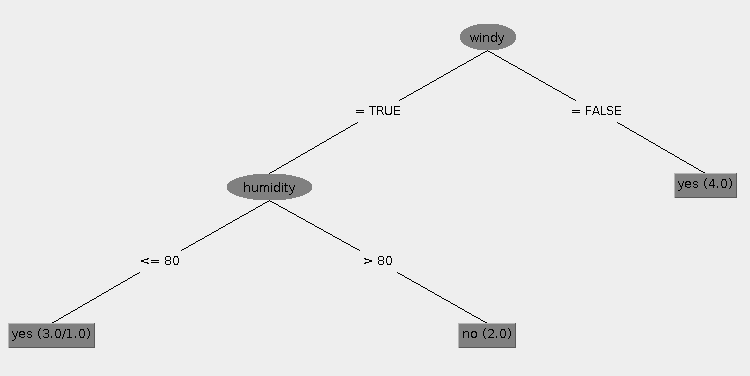
\includegraphics[width=0.8\textwidth]{ArbreSeuil.png}
	    \caption{Arbre de décision avec attributs numériques}
	    \label{fig:ArbreSeuil} 
	  \end{center}
	\end{figure}

\end{enumerate}


\section{Elagage et simplification}

\begin{enumerate}
\item En supprimant l'élagage, l'arbre possède plus de noeuds et de feuilles.
Le nombre d'exemples bien classés est de 60\% par rapport aux 40\% de l'arbre élagué. 

Nos résultats pratiques ne semblent pas cohérents. En effet, l'arbre élagué est plus général, il devrait donc être plus performant que le non élagué.

\item Un exemple d'arbre possédant 3 objets par feuille est visible en figure~\ref{fig:ArbreSeuilNonElag}. Avec plus d'objets par feuille l'arbre est moins grand, il possède moins de feuilles et de noeuds. Les résultat obtenus montrent que le classifieurs possédant 3 objets minimum par feuille est moins efficace avec 40\% d'exemples bien classés seulement.

    
\begin{figure}[h]
  \begin{center}
    \begin{minipage}[t]{0.48\textwidth}
		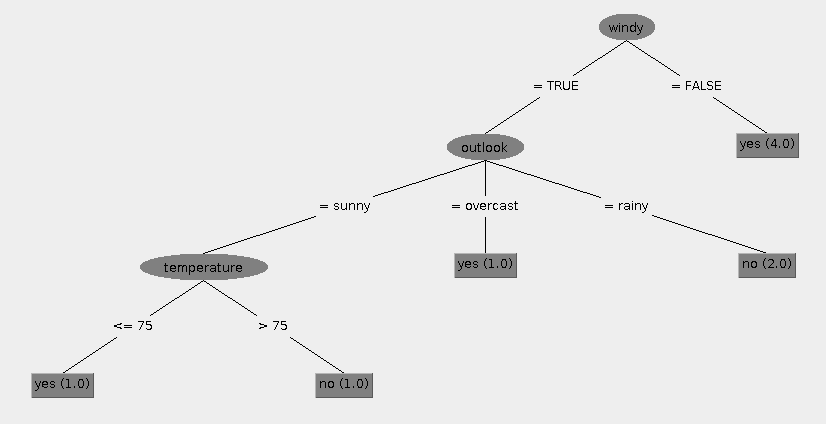
\includegraphics[width=0.9\textwidth]{ArbreNonElage.png}
	    \caption{Arbre non élagué}
	    \label{fig:ArbreSeuil} 
    \end{minipage}
    \hfill
    \begin{minipage}[t]{0.48\textwidth}
		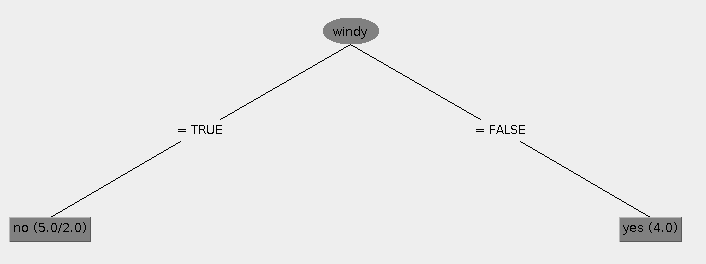
\includegraphics[width=0.9\textwidth]{ArbreNonElage3Obj.png}
	    \caption{Arbre non élagué à 3 objets minimum par feuille}
	    \label{fig:ArbreSeuilNonElag}
    \end{minipage}
  \end{center}
\end{figure}


\end{enumerate}

\section{Apprentissage bayésien}
\subsection{Bayes Naïf}

\begin{enumerate}

\item L'hypothèse naïve utilisée ici est que tous les attributs (\textit{outlook}, \textit{temperature}, \textit{humidity}, \textit{windy}, \textit{play})  sont indépendants.
Cette hypothèse permet d'obtenir la relation p(x|w) = $\prod_{i}$ p($a_{i}$), où w est la classe, x un exemple et $a_{i}$ sont les différents attributs.

\item Weka estime pour chaque classe la répartition des attributs selon les classes. Pour les attributs numériques, il calcule la répartition selon une loi normale. Weka estime donc les proba a-posteriori.

On constate que Weka utilise l'estimation de Laplace, pour éviter d'avoir un numérateur égal à 0. Ainsi, on ajoute à chaque valeur au numérateur et au dénominateur.

\item On cherche :
$p([Ensoleille, 73, 81, Fort]|yes)$ et $p([Ensoleille, 73, 81, Fort]|yes)$.

$p([Ensoleille, 73, 81, Fort]|yes) = p(Ensoleille|yes) * p (73|yes) * p(81|yes) * p(Fort|yes) 
= 2/9 * 0.07627 * 0.03972 * 3/9 
=  0.000224423$

$p([Ensoleille, 73, 81, Fort]|no) 
= p(Ensoleille|no) * p (73|no) * p(81|no) * p(Fort|no) 
= 0.000698566$

La classe choisie sera donc "no", selon la règle du maximum de vraisemblance.

Nous vérifions le résultat avec Weka, en insérant la donnée demandée comme donnée de test

\begin{lstlisting}[frame=single]
@relation weather

@attribute outlook{sunny,overcast,rainy}
@attribute temperature real
@attribute humidity real
@attribute windy {TRUE, FALSE}
@attribute play {yes, no}

@data
sunny, 73, 81, TRUE, no
\end{lstlisting}

Le résultat de Weka corrobore notre calcul théorique. 

\begin{lstlisting}[frame=single]
=== Evaluation result ===

Scheme: NaiveBayes
Relation: weather


Correctly Classified Instances           1              100      %
Incorrectly Classified Instances         0                0      %
Kappa statistic                          1     
Mean absolute error                      0.4225
Root mean squared error                  0.4225
Relative absolute error                126.7442 %
Root relative squared error            126.7442 %
Total Number of Instances                1     

=== Detailed Accuracy By Class ===

TP Rate   FP Rate   Precision   Recall  F-Measure   ROC Area  Class
  0         0          0         0         0          ?        yes
  1         0          1         1         1          ?        no

=== Confusion Matrix ===

 a b   <-- classified as
 0 0 | a = yes
 0 1 | b = no
\end{lstlisting}

Celui-ci classe bien la donnée comme appartenent à la classe "no". Il n'y aura donc pas de jeu !

\item Nous allons utiliser les arbres de décisions pour comparer les résultats. Nous utilisons les données fournies en données d'entrainement et nous utilisons le fichier contenant uniquement la valeur à vérifier en données de test. Le résultat obtenu est le même, la donnée de test est classifiée en "no".

\begin{lstlisting}[frame=single]
=== Evaluation result ===

Scheme: J48
Relation: weather


Correctly Classified Instances           1              100      %
Incorrectly Classified Instances         0                0      %
Kappa statistic                          1     
Mean absolute error                      0     
Root mean squared error                  0     
Relative absolute error                  0      %
Root relative squared error              0      %
Total Number of Instances                1     

=== Detailed Accuracy By Class ===

TP Rate   FP Rate   Precision   Recall  F-Measure   ROC Area  Class
  0         0          0         0         0          ?        yes
  1         0          1         1         1          ?        no

=== Confusion Matrix ===

 a b   <-- classified as
 0 0 | a = yes
 0 1 | b = no
\end{lstlisting}

\end{enumerate}

\subsection{Approche non paramétrique}

\begin{enumerate}

\item L'algorithme IBk est l'algorithme des K-plus proches voisins. Afin de trouver la classe d'un objet, on regarde les k points les plus proches de l'objet à classifier. On attribut alors à l'objet la classe qui apparaît le plus dans ses k voisins.

\item On utilise l'algorithme IB1 sur les données de  \emph{iris.arff}. On utilise un \emph{TrainTestSplitMarker} afin de s'entrainer sur 66\% des données et de tester avec les 33\% autres. On obtient le résultat suivant.

\begin{lstlisting}[frame=single]
=== Evaluation result ===

Scheme: IB1
Relation: iris


Correctly Classified Instances          49               96.0784 %
Incorrectly Classified Instances         2                3.9216 %
Kappa statistic                          0.9408
Mean absolute error                      0.0261
Root mean squared error                  0.1617
Relative absolute error                  5.9081 %
Root relative squared error             34.3789 %
Total Number of Instances               51     

=== Detailed Accuracy By Class ===

TP Rate   FP Rate   Precision   Recall  F-Measure   ROC Area  Class
  1         0          1         1         1          1        Iris-setosa
  1         0.063      0.905     1         0.95       0.969    Iris-versicolor
  0.882     0          1         0.882     0.938      0.941    Iris-virginica

=== Confusion Matrix ===

  a  b  c   <-- classified as
 15  0  0 |  a = Iris-setosa
  0 19  0 |  b = Iris-versicolor
  0  2 15 |  c = Iris-virginica
\end{lstlisting}

On constate que seulement 2 fleurs n'ont pas été classées correctement sur les 51, soit un taux d'erreur de 4\%. Les résultats sont donc satisfaisants.

\item L'utilisation d'un algorithme IB2 donne exactement les mêmes résultats.

\item Afin de choisir un K minimisant les erreurs, il existe une heuristique indiquant que : $K =  \sqrt{m/c}$.


Ici, on obtient : $K = \sqrt{51/3} = 4$

On teste donc avec un algorithme IB4. Les résultats obtenues sont strictement les mêmes qu'avec IB1 et IB2.
Dans notre exemple, le choix de K ne permet pas d'affiner le résultat car l'algorithme est déjà efficace avec K=1 sur ce jeu de données.
\end{enumerate}


\end{document}